\section{Resultados}
\label{sec:results}

Os resultados obtidos levam em consideração a quantidade de casos que houveram convergência, e dentre esses casos, a quantidade de iterações necessárias. As informações são apresentadas de forma comparativa com o método Newton nos mesmos cenários de convergência. Todos os testes de convergência possuem um limite de 50 iterações, ao ultrapassá-lo é assumido que o algoritmo não convergiu. 

\subsection{Variando Uma Variável}
\label{sec:res-one-var}

Para os cenários onde uma variável de cada vez era afastado de seu estado otimizado, foi feita uma análise da taxa de sucesso de convergência por ponto estacionário como apresentado no gráfico \ref{fig:result-one-var-conv-tax}. Para os casos de sucesso de convergência, um gráfico de dispersão foi montado apresentando o percentual da quantidade de casos de convergência por número de iterações necessárias conforme apresentado no gráfico \ref{fig:result-one-var-conv-metric}.

\begin{figure}[h]
  \begin{subfigure}{.5\textwidth}
    \begin{center}
      \begin{center}
  
  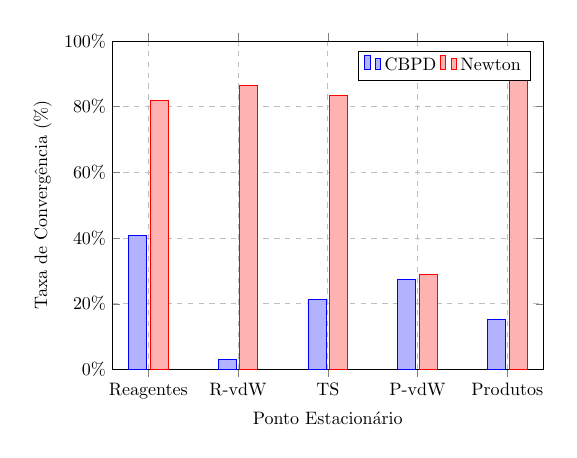
\begin{tikzpicture}[scale = 0.65]
    \begin{axis}[
      width=10cm,
      height=8cm,
      xlabel={Ponto Estacionário},
      ylabel={Taxa de Convergência (\%)},
      xtick=data,
      xticklabels={Reagentes, R-vdW, TS, P-vdW, Produtos},
      legend style={at={(0.5,-0.2)}, anchor=north, legend columns=-1},
      ymin=0,
      ymax=100,
      grid=major,
      grid style=dashed,
      ymajorgrids=true,
      ybar,
      ytick={0,20,...,100},
      yticklabel={\pgfmathprintnumber{\tick}\%},
      legend pos=north east
    ]

      \addplot[color=blue, fill=blue!30] coordinates {
        (1, 40.91)
        (2, 3.03)
        (3, 21.21)
        (4, 27.27)
        (5, 15.15)
      };

      \addplot[color=red, fill=red!30] coordinates {
        (1, 81.82)
        (2, 86.36)
        (3, 83.33)
        (4, 28.79)
        (5, 93.94)
      };

      \legend{CBPD, Newton}

    \end{axis}
  \end{tikzpicture}

\end{center}

    \end{center}
    \caption{Taxa de sucesso de convergência para os métodos iterativos CBPD e Newton para cada ponto estacionário da reação \ce{F + H2O -> FH + HO} nos casos de variação de uma variável.}
    \label{fig:result-one-var-conv-tax}
  \end{subfigure}\hspace{5mm}%
  \begin{subfigure}{.5\textwidth}
    \begin{center}
      \begin{center}
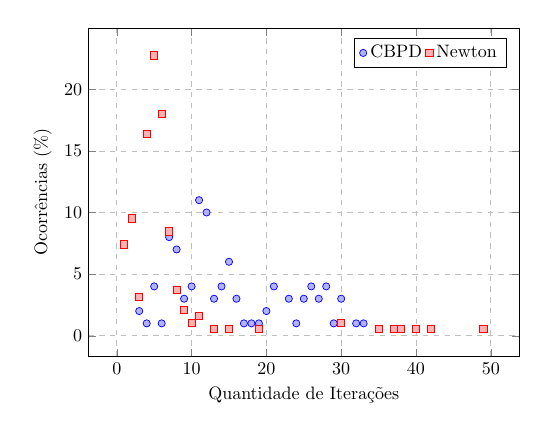
\begin{tikzpicture}[scale = 0.65]
  \begin{axis}[
    width=10cm,
    height=8cm,
    xlabel={Quantidade de Iterações},
    ylabel={Ocorrências (\%)},
    legend style={at={(0.5,-0.2)}, anchor=north, legend columns=-1},
    grid=major,
    grid style=dashed,
    legend pos=north east
  ]

    % First set of data
    \addplot[
      only marks,
      mark=*,
      color=blue,
      fill=blue!30,
    ] coordinates {
        (12, 10.00)
        (11, 11.00)
        (5, 4.00)
        (13, 3.00)
        (14, 4.00)
        (15, 6.00)
        (9, 3.00)
        (7, 8.00)
        (23, 3.00)
        (16, 3.00)
        (8, 7.00)
        (30, 3.00)
        (32, 1.00)
        (19, 1.00)
        (33, 1.00)
        (21, 4.00)
        (20, 2.00)
        (25, 3.00)
        (26, 4.00)
        (28, 4.00)
        (27, 3.00)
        (29, 1.00)
        (10, 4.00)
        (18, 1.00)
        (17, 1.00)
        (24, 1.00)
        (6, 1.00)
        (4, 1.00)
        (3, 2.00)
      };

    % Second set of data
    \addplot[
      only marks,
      mark=square*,
      color=red,
      fill=red!30,
    ] coordinates {
        (6, 17.99)
        (5, 22.75)
        (4, 16.40)
        (2, 9.52)
        (7, 8.47)
        (3, 3.17)
        (9, 2.12)
        (8, 3.70)
        (10, 1.06)
        (11, 1.59)
        (35, 0.53)
        (38, 0.53)
        (40, 0.53)
        (30, 1.06)
        (13, 0.53)
        (1, 7.41)
        (15, 0.53)
        (49, 0.53)
        (42, 0.53)
        (37, 0.53)
        (19, 0.53)
    };
    \legend{CBPD, Newton}

  \end{axis}
\end{tikzpicture}
\end{center}

    \end{center}
    \caption{Percentual da quantidade de iterações necessárias para convergir para os métodos iterativos CBPD e Newton para a reação \ce{F + H2O -> FH + HO} nos casos de variação de uma variável.}
    \label{fig:result-one-var-conv-metric}
  \end{subfigure}
  \caption{Resultados dos casos de variação de uma variável.}
\end{figure}

\subsection{Cenários Aleatórios de Convergência}

Para os cenários de convergência nos quais todas as variáveis são aleatorizadas, foi feita uma análise similar à descrita na seção \ref{sec:res-one-var}. Uma análise da taxa de convergência por ponto estacionário é apresentada no gráfico \ref{fig:result-mult-var-conv-tax}, enquanto para os casos de sucesso convergência, um gráfico de dispersão foi montado apresentando o percetual da quantidade de casos de convergência por número de interações conforme apresentado no gráfico \ref{fig:result-mult-var-conv-metric}.

\begin{figure}[h]
  \begin{subfigure}{.5\textwidth}
    \begin{center}
    \begin{center}
  
  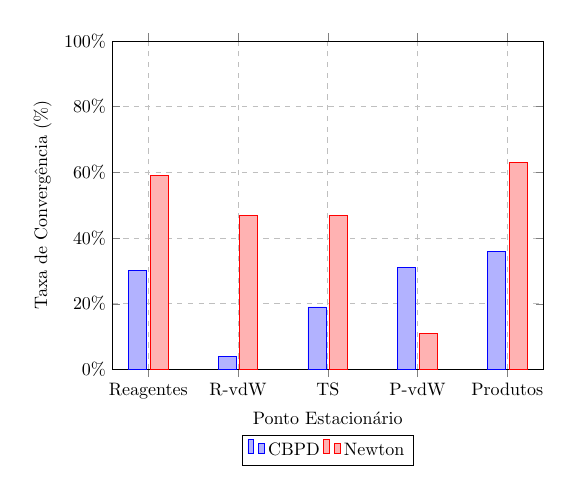
\begin{tikzpicture}[scale = 0.65]
    \begin{axis}[
      width=10cm,
      height=8cm,
      xlabel={Ponto Estacionário},
      ylabel={Taxa de Convergência (\%)},
      xtick=data,
      xticklabels={Reagentes, R-vdW, TS, P-vdW, Produtos},
      legend style={at={(0.5,-0.2)}, anchor=north, legend columns=-1},
      ymin=0,
      ymax=100,
      grid=major,
      grid style=dashed,
      ymajorgrids=true,
      ybar,
      ytick={0,20,...,100},
      yticklabel={\pgfmathprintnumber{\tick}\%}
    ]

      \addplot[color=blue, fill=blue!30] coordinates {
        (1, 30.00)
        (2, 4.00)
        (3, 19.00)
        (4, 31.00)
        (5, 36.00)
      };

      \addplot[color=red, fill=red!30] coordinates {
        (1, 59.00)
        (2, 47.00)
        (3, 47.00)
        (4, 11.00)
        (5, 63.00)
      };

      \legend{CBPD, Newton}

    \end{axis}
  \end{tikzpicture}

\end{center}

    \end{center}
    \caption{Taxa de sucesso de convergência para os métodos iterativos CBPD e Newton para cada ponto estacionário da reação \ce{F + H2O -> FH + HO} nos cenários aleatórios de convergência.}
    \label{fig:result-mult-var-conv-tax}
  \end{subfigure}\hspace{5mm}%
  \begin{subfigure}{.5\textwidth}
    \begin{center}
    \begin{center}
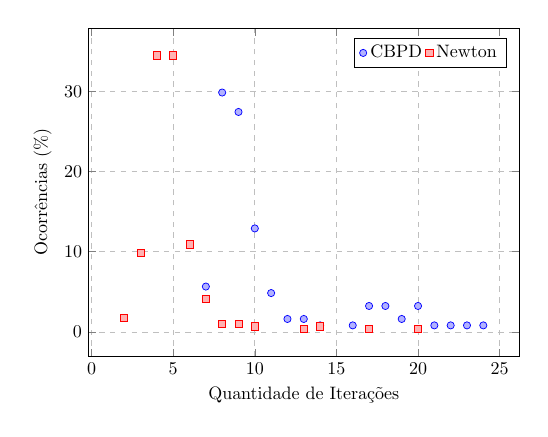
\begin{tikzpicture}[scale = 0.65]
  \begin{axis}[
    width=10cm,
    height=8cm,
    xlabel={Quantidade de Iterações},
    ylabel={Ocorrências (\%)},
    legend style={at={(0.5,-0.2)}, anchor=north, legend columns=-1},
    grid=major,
    grid style=dashed,
    legend pos=north east
  ]

    % First set of data
    \addplot[
      only marks,
      mark=*,
      color=blue,
      fill=blue!30,
    ] coordinates {
        (9, 27.42)
        (10, 12.90)
        (8, 29.84)
        (7, 5.65)
        (11, 4.84)
        (13, 1.61)
        (12, 1.61)
        (18, 3.23)
        (20, 3.23)
        (23, 0.81)
        (24, 0.81)
        (22, 0.81)
        (17, 3.23)
        (19, 1.61)
        (14, 0.81)
        (21, 0.81)
        (16, 0.81)
      };

    % Second set of data
    \addplot[
      only marks,
      mark=square*,
      color=red,
      fill=red!30,
    ] coordinates {
        (4, 34.47)
        (5, 34.47)
        (3, 9.90)
        (2, 1.71)
        (6, 10.92)
        (8, 1.02)
        (7, 4.10)
        (10, 0.68)
        (17, 0.34)
        (13, 0.34)
        (9, 1.02)
        (14, 0.68)
        (20, 0.34)
    };
    \legend{CBPD, Newton}

  \end{axis}
\end{tikzpicture}
\end{center}

    \end{center}
    \caption{Percentual da quantidade de iterações necessárias para convergir para os métodos iterativos CBPD e Newton para a reação \ce{F + H2O -> FH + HO} nos cenários aleatórios de convergência.}
    \label{fig:result-mult-var-conv-metric}
  \end{subfigure}
  \caption{Resultados dos cenários aleatórios de convergência.}
\end{figure}

Avaliando as taxas de convergências dos métodos CBPD e Newton é notório que o método de Newton apresenta melhores resultados de convergência na maioria dos pontos estacionários da reação com exceção do $P-vdW$. Em termos de quantidades de iterações necessárias para convergência, o Método de Newton apresenta uma maior consistência, sendo necessário em torno de 5 a 7 iterações. Já no Método CBPD a quantidade de iterações necessárias possui um pico entre 11 e 12 iterações.
